\subsection{Travaux préliminaires}
\begin{frame}[c]{Travaux préliminaires}
    \vfill
    \begin{columns}[c,totalwidth=\textwidth]
        \column{0.54\textwidth}
        \begin{itemize}
            \item \citeauthortitle{boegeat_rapport_2023-1} : structure d’accroche Crazyflie imprimée 3D avec aimants
            \item \citeauthortitle{boegeat_rapport_2023} : amélioration du système, documentation
            \item \citeauthortitle{bonnel_modeling_2024} : modélisation de deux quadricoptères couplés (équivalent octocoptère)
        \end{itemize}

        \column{0.4\textwidth}
        \begin{figure}
            \centering
            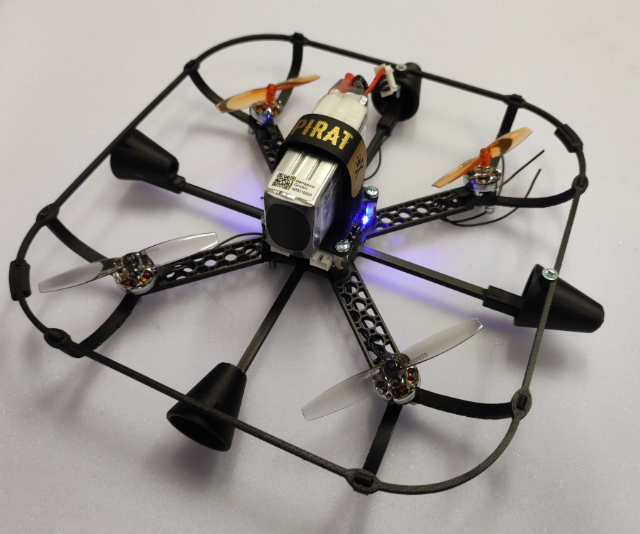
\includegraphics[width=\linewidth]{3-etat-de-lart/travaux_preli/pic/crazyflie_structure.PNG}
            \caption{Crazyflie eSWARM}
            \label{fig:crazyflie_struct}
        \end{figure}
    \end{columns}
    \vfill
\end{frame}
